\documentclass{article}%
\usepackage[T1]{fontenc}%
\usepackage[utf8]{inputenc}%
\usepackage{lmodern}%
\usepackage{textcomp}%
\usepackage{lastpage}%
\usepackage[head=40pt,margin=0.5in,bottom=0.6in]{geometry}%
\usepackage{graphicx}%
%
\title{\textbf{Registran en más de 5.000.000\% inflación durante seis años en Venezuela}}%
\author{DICK TORRES}%
\date{07/03/2019}%
%
\begin{document}%
\normalsize%
\maketitle%
\textbf{URL: }%
http://www.eluniversal.com/economia/34968/registran{-}en{-}5{-}millardos{-}inflacion{-}durante{-}seis{-}anos\newline%
%
\textbf{Periodico: }%
EU, %
ID: %
34968, %
Seccion: %
economia\newline%
%
\textbf{Palabras Claves: }%
NO\_TIENE\newline%
%
\textbf{Derecho: }%
2.1%
, Otros Derechos: %
\newline%
%
\textbf{\textit{El diputado Elías Matta dijo que ningún salario puede soportar la hiperinflación}}%
\newline%
\newline%
%
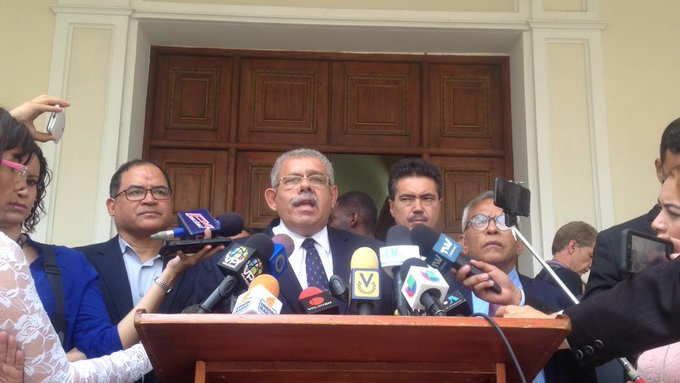
\includegraphics[width=300px]{EU_34968.jpg}%
\newline%
%
Caracas.{-}~En 5.395.536.286\% esa es la inflación acumulada durante los seis años de gobierno del presidente Nicolás Maduro, según cálculos del diputado Elías Matta.%
\newline%
%
El parlamentario cerró este miércoles el debate de la Asamblea Nacional (AN) sobre “la acelerada crisis económica y sus efectos en la población” provocada por la administración de Maduro.%
\newline%
%
Matta, presidente de la Comisión de Energía y Minas, expresó que ante esos indicadores  económicos “no existe ningún salario que pueda soportar semejante presión inflacionaria”.%
\newline%
%
Observó que durante 20 años de gobierno socialista se han producido 46 aumentos de salarios, 26 de los cuales han sido dictados por la administración de Maduro, de quien refirió anuncia otro incremento salarial, “pero para qué han servido esos aumentos, sino se ataca la hiperinflación”, reclamó.%
\newline%
%
Recordó que en 2013, Maduro juró ante la AN que su gobierno daría un giro en materia de control de cambio y en el tema petrolero entre otros compromisos, pero “lo que hizo fue profundizar la crisis económica venezolana”.%
\newline%
%
Comentó que de acuerdo a los datos aportados por la Comisión de Finanzas de la AN, la inflación en Venezuela crece diariamente 3,5\%.%
\newline%
%
El parlamentario comparó esa cifra con los índices de inflación en Ecuador donde anualmente su crecimiento se ubica en 0,37\%.%
\newline%
%
“Y en Bolivia, uno de los aliados de Maduro, la inflación anual es de 1,52\%, mientras que en \_Venezuela la inflación crece, cada 24 horas 3,5\%”, dijo.%
\newline%
%
Según el diputado, no se puede entender cómo un país que depende del 95\% de sus ingresos petroleros, su principal industria “sea hoy un desastre”.%
\newline%
%
Hizo referencia a un informe reciente de la Organización de países Exportadores de Petróleo (OPEP), según el cual Venezuela dejó de percibir 32.432 millones de dólares por la caída de su producción estimada en 1.7 millones de barriles diarios al precio de 54 dólares.%
\newline%
%
En cuanto al Producto Interno Bruto (PIB) expresó que ha sufrido una caída del 56\%.%
\newline%
%
“En el tema del crecimiento económico durante estos últimos seis años de gobierno se ha perdido, no porque el país haya sufrido una catástrofe natural o una guerra como en Siria, sino por las malas políticas de un gobierno ineficiente e incapaz”, agregó.%
\newline%
%
Matta afirmó que durante el lapso 2016 {-} 2019 el país tuvo ingresos por 917.491 millones de dólares, según datos oficiales del Banco Central de Venezuela (BCV) “que fueron desaprovechados debido a que el Gobierno multiplicó por seis la deuda pública”, agregó.%
\newline%
%
Denunció que el Fondo para el Desarrollo Nacional (Fonden), entidad creada por el Gobierno en 2005 para invertir los ingresos producto de las exportaciones del petróleo, no existe informe sobre los recursos que ha recibido por el orden de los 143.573 millones de dólares.%
\newline%
%
Plan País%
\newline%
%
Matta dijo que la oposición y el equipo económico de Juan Guaidó han propuesto como solución a la crisis el “Plan País”, con el objetivo de reactivar la industria petrolera y derrotar la inflación.%
\newline%
%
Durante el debate parlamentario, intervino inicialmente el diputado José Guerra quien expresó que  el tema económico es altamente sensible para el pueblo venezolano que está “arruinado por los efectos destructivo de la hiperinflación”.%
\newline%
%
A su juicio el salario mínimo en Venezuela es 5,45 dólares al mes, “el más bajo del planeta”.%
\newline%
%
Por su parte, el diputado Carlos Prosperi dijo que un ciudadano estadounidense gana diariamente entre 9 a 12 dólares que equivalen a menos de un salario mensual para un trabajador de venezolano.%
\newline%
%
dicktorres@gmail.com%
\newline%
%
\end{document}